\documentclass[table,dvipsnames]{beamer}
\mode<presentation>{
	\usetheme{Madrid}
	\setbeamercolor{title}{fg=Black,bg=Blue!15}
	\setbeamercolor{frametitle}{fg=Black,bg=Blue!15}
	\setbeamercolor{block title}{fg=Black,bg=Blue!15}
	\setbeamercolor{block}{fg=Black,bg=Blue!10}
}

%\usepackage{default}
\usepackage{graphicx}
\usepackage{booktabs}
\usepackage{xcolor}
\usepackage{multirow}
\usepackage{minted}
\usepackage[
type={CC},
modifier={by-sa},
version={4.0},
]{doclicense}

\definecolor{LightGray}{gray}{0.9}

\title[Devs Beginner Guide]{Briefing Devs for Beginner}
\author{}
\date{}

\begin{document}

	\section{Start}

	\begin{frame}
	\titlepage
	\end{frame}

	\begin{frame}
		\frametitle{Disclaimer}
		\begin{exampleblock}{}
			These activities are NOT lecture or workshop activity in regular way
		\end{exampleblock}
		\begin{exampleblock}{}
			These activities are self training using prepared guideline documents 	
		\end{exampleblock}
		\begin{exampleblock}{}
			Learning by doing is the best learning way
			\begin{center}
				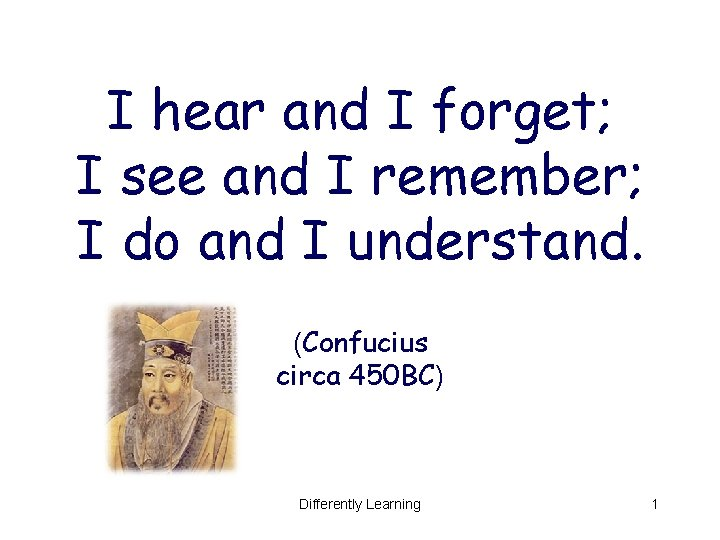
\includegraphics[width=150pt]{images/confucius}
			\end{center}
		\end{exampleblock}
	\end{frame}

	\begin{frame}
		\frametitle{Contents: Why-ies}
		\begin{exampleblock}{}
			Why need Linux ?
		\end{exampleblock}
		\begin{exampleblock}{}
			Why need Git ?
		\end{exampleblock}
		\begin{exampleblock}{}
			Why need Github ?
		\end{exampleblock}
	\end{frame}	

	\begin{frame}
		\frametitle{Why need Linux}
		\begin{exampleblock}{}
			RaspberryPi and many single-board computer run on Linux distros
			\begin{center}
				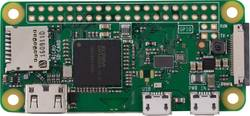
\includegraphics[width=150pt]{images/rpizerow}
			\end{center}
		\end{exampleblock}
		\begin{exampleblock}{}
			Some of popular Linux variant:
			\begin{itemize}
				\item RaspberryPi OS \\
				\url{https://www.raspberrypi.org/software/}
				
				\item Ubuntu Mate Raspberry \\
				\url{https://ubuntu-mate.org/raspberry-pi/}
				
				\item Arch Linux ARM \\
				\url{https://archlinuxarm.org/}
			\end{itemize}
		\end{exampleblock}
		
	\end{frame}

\end{document}